% !TEX program = xelatex
\documentclass[11pt,a4paper,fontset=windows]{ctexart}
\usepackage[a4paper,margin=2.4cm]{geometry}
\usepackage{amsmath,amssymb}
\usepackage{graphicx}
\usepackage{booktabs}
\usepackage{float}
\usepackage{xcolor}
\usepackage[colorlinks=true,linkcolor=blue!60!black,citecolor=blue!60!black]{hyperref}
\graphicspath{{figures/}}

\definecolor{accent}{RGB}{170,110,255}

\title{\textbf{DR 光凝标注派生结构算法说明}\\[2mm]\large LabelMyEye --- 视盘 / 黄斑 / 血管弓区 / 后极部 / 光凝敏感区}
\author{LabelMyEye 项目}
\date{2026 年 9 月}

\begin{document}
\maketitle

\begin{abstract}
本文档完整描述 LabelMyEye 中糖尿病视网膜病变（DR）光凝标注五个派生结构的计算方法：
输入由点击式分割（MobileSAM）得到的视盘圆与黄斑圆，随后确定性派生血管弓区椭圆
（macular\_area）、后极部边界（posterior\_pole\_boundary）与光凝敏感区
（central\_inner）。所有默认参数由组内 14 例手绘标注经最小二乘拟合标定。
实现位于 \texttt{labelmyeye/dr\_geometry.py}；插图由
\texttt{scripts/make\_algorithm\_figures.py} 生成。
\end{abstract}

\section{总览与约定}

\begin{figure}[H]\centering
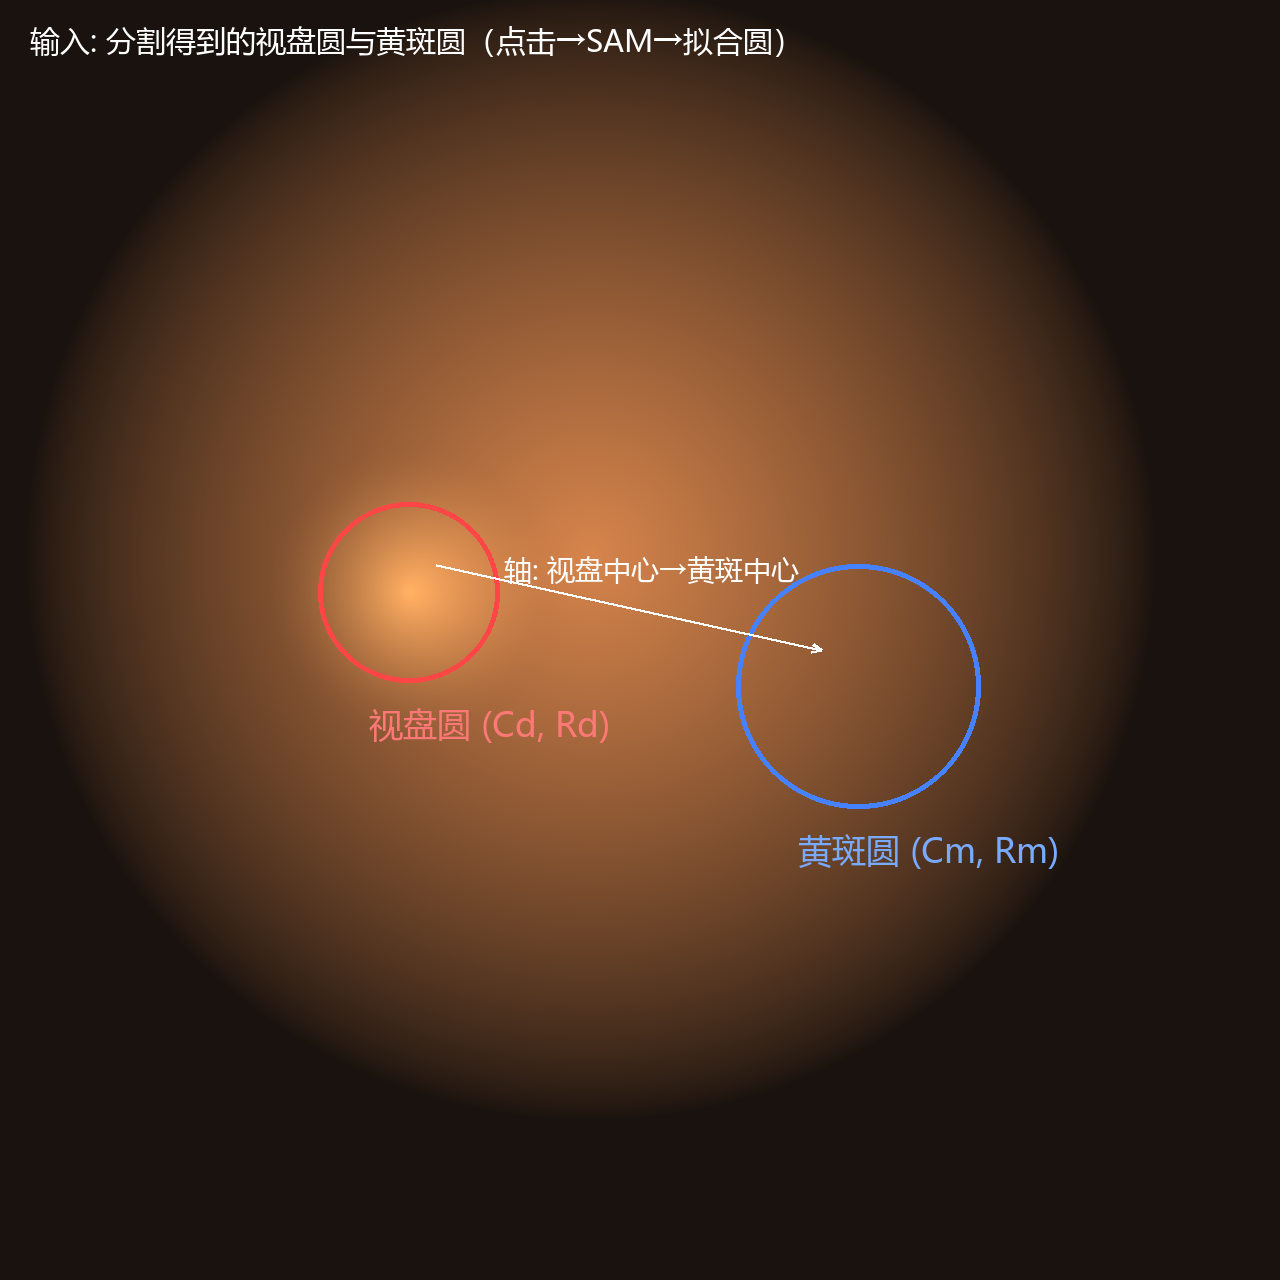
\includegraphics[width=0.82\linewidth]{fig1_input.png}
\caption{算法输入：分割得到的视盘圆 $(C_d, R_d)$ 与黄斑圆 $(C_m, R_m)$，
以及视盘中心$\to$黄斑中心的轴线。}
\end{figure}

\paragraph{单位约定}全文 1\,PD（视盘直径）$= 2 R_d$（$R_d$ 为视盘半径）。
算法内部以像素计算，参数以 PD 表述。

\paragraph{派生流程}两个输入圆齐备后，一次性派生五个结构：
\texttt{optic}（视盘圆）、\texttt{macular}（黄斑圆）、\texttt{macular\_area}（绿椭圆）、
\texttt{posterior\_pole\_boundary}（橙卵圆）、\texttt{central\_inner}（紫肾形）。
五者共享同一 \texttt{group\_id}，便于整体管理与重算。

\section{macular\_area：相切两圆的血管弓区椭圆}

解剖学上对应颞侧血管弓围住的区域。构造规则（函数
\texttt{tangent\_ellipse\_two\_circles}）：

\begin{enumerate}
\item 长轴方向取视盘中心 $C_d$ 指向黄斑中心 $C_m$ 的连线方向 $\mathbf u$；
\item 椭圆两端顶点恰好落在视盘圆的鼻侧极点
$P_1 = C_d - R_d\,\mathbf u$ 与黄斑圆的颞侧极点
$P_2 = C_m + R_m\,\mathbf u$，因此与两个圆同时相切（图~\ref{fig:ell}）；
\item 中心 $E = (P_1+P_2)/2$，长半轴 $a = |P_2-P_1|/2$；
\item 短半轴 $b$ 取"恰好完整包住两个圆"的最小值（数值二分求解）。
\end{enumerate}

\begin{figure}[H]\centering
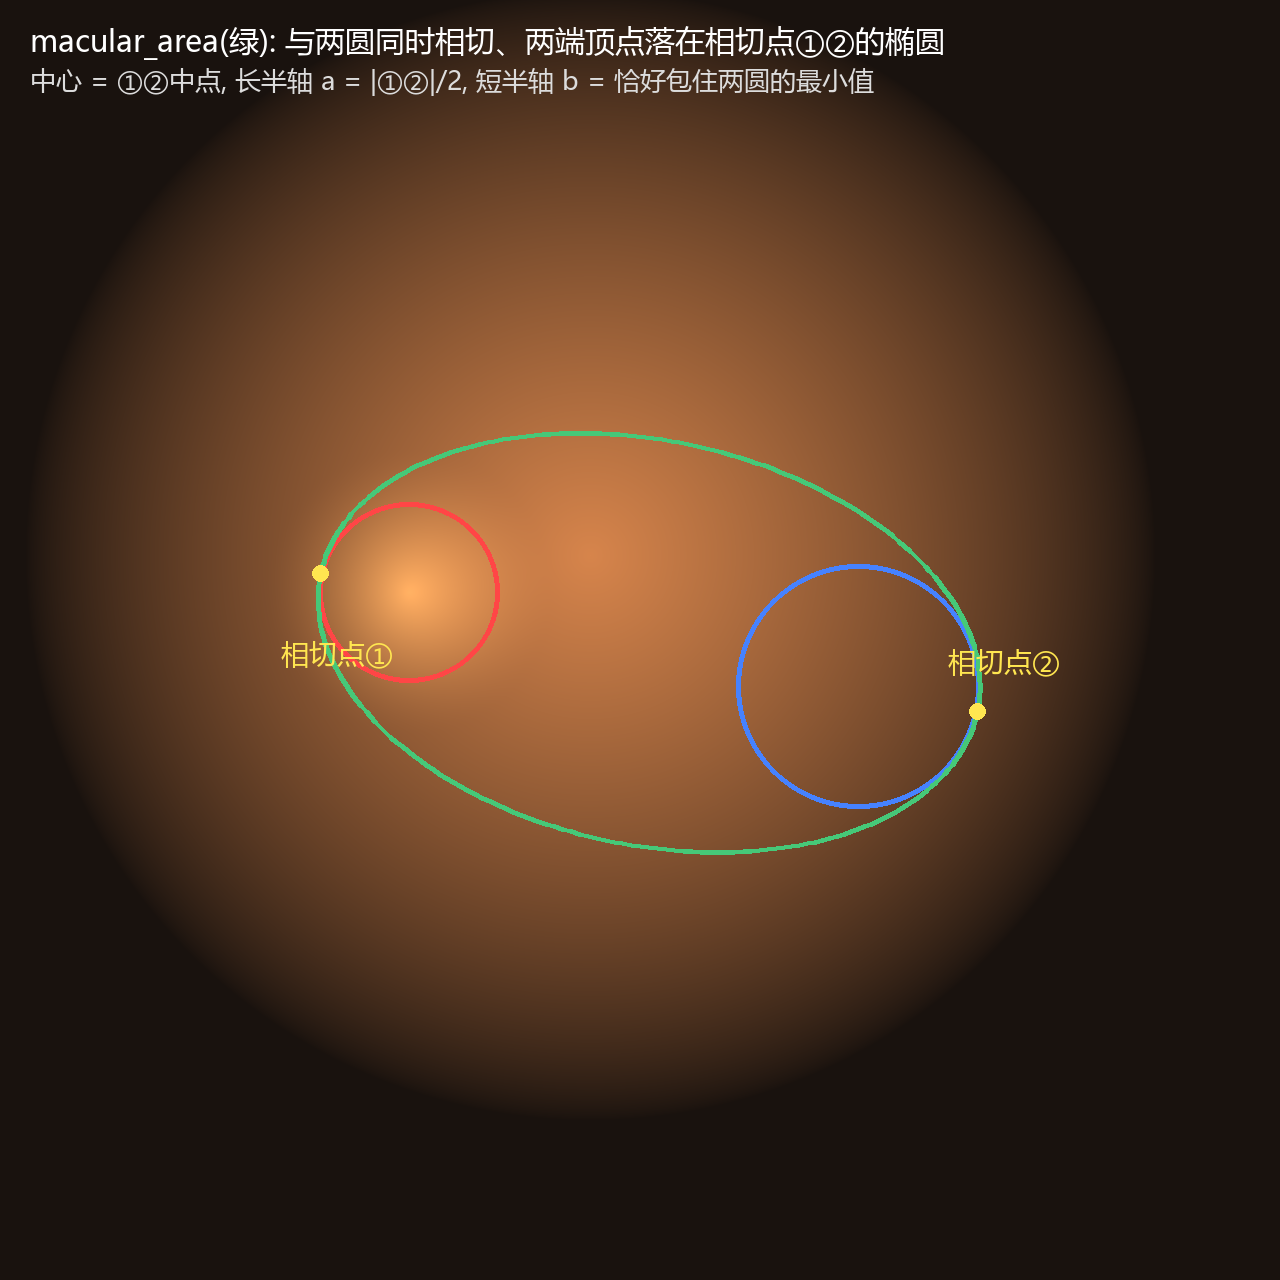
\includegraphics[width=0.82\linewidth]{fig2_tangent.png}
\caption{绿椭圆与两圆相切：两端顶点分别落在相切点①②。}
\label{fig:ell}
\end{figure}

该构造是确定性的：同一对输入圆永远得到同一椭圆。

\section{posterior\_pole\_boundary：后极部边界（不对称卵圆）}

以绿椭圆\textbf{边缘}为基准向外推，不同方向推的距离不同：

\begin{center}
\begin{tabular}{lll}
\toprule
方向 & 外扩量 & 说明 \\
\midrule
颞侧（黄斑侧） & 2\,PD & 沿长轴向黄斑方向 \\
鼻侧（视盘侧） & 1\,PD & 沿长轴向视盘方向 \\
上 / 下 & 各 2\,PD & 沿短轴方向 \\
\bottomrule
\end{tabular}
\end{center}

颞、鼻外扩量不同，故结果为\textbf{不对称卵圆}：颞半椭圆
（半轴 $a_t = a + 2\mathrm{PD}$，$b_v = b + 2\mathrm{PD}$）与鼻半椭圆
（半轴 $a_n = a + 1\mathrm{PD}$，$b_v$ 同）在上下顶点拼合。

\begin{figure}[H]\centering
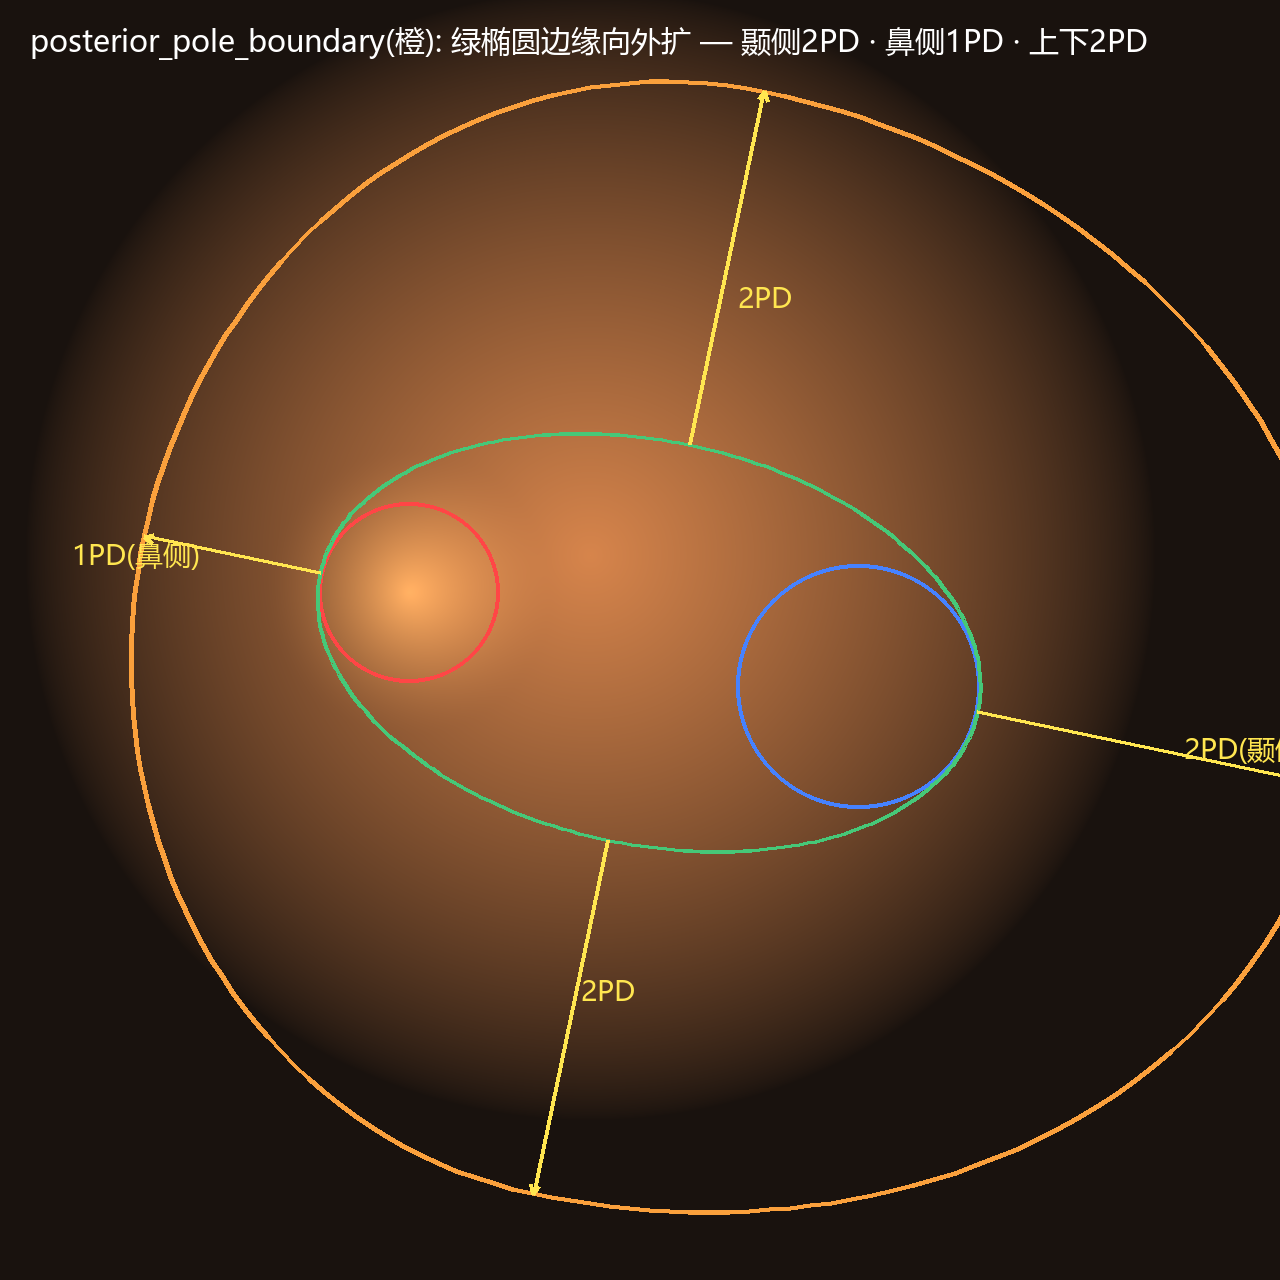
\includegraphics[width=0.8\linewidth]{fig3_pp.png}
\caption{后极部边界（橙）：绿椭圆边缘向外——颞侧 2PD、鼻侧 1PD、上下 2PD。}
\end{figure}

\section{central\_inner：光凝敏感区（径向轮廓法)}

光凝敏感区表示\textbf{必须避开的区域}：后极部整体，但需在上下两个方向"让开"——
乳头黄斑束两侧、血管弓之外是允许打激光的区域（PRP 施加处）。

\subsection{径向轮廓法}

以后极部卵圆中心 $E$ 为原点，沿 96 个方向 $\varphi$ 各计算一个边界距离
$r(\varphi)$，连成闭合多边形。整个形状由一个径向函数完全描述：

\begin{equation}
r(\varphi) \;=\; \max\Big(\, R_{pp}(\varphi)\,\bigl(1 - d(\varphi)\bigr),\;\;
r_{bub}(\varphi) \,\Big)
\label{eq:main}
\end{equation}

其中三项分别见下。

\subsection{$R_{pp}(\varphi)$：外极限轮廓}

$E$ 到后极部卵圆边界在该方向上的距离（解析式：
$r = a\,b \,/\, \sqrt{(b\cos\delta)^2 + (a\sin\delta)^2}$，
$\delta$ 为相对长轴的角度，颞半取 $a_t$、鼻半取 $a_n$）。
它给出"贴住后极部"的外极限——轮廓永远不会超过它。

\subsection{高斯凹口 $d(\varphi)$：让出上下激光安全区}

\begin{equation}
d(\varphi) \;=\; \max\Big(
d_{sup}\, e^{-\frac{(\varphi - a_{sup})^2}{2\sigma^2}},\;\;
d_{inf}\, e^{-\frac{(\varphi - a_{inf})^2}{2\sigma^2}} \Big)
\label{eq:depth}
\end{equation}

凹口中心 $a_{sup} = +123^\circ$、$a_{inf} = -128^\circ$（相对轴线，
偏向鼻侧——血管弓离开视盘的方位），深度 $d_{sup}=0.50$、$d_{inf}=0.46$，
平滑度 $\sigma = 40^\circ$。在凹口正中，边界收缩到后极部的
$1-d_{sup} = 50\%$；偏离 $\pm\sigma$ 处剩余 61\%；$\pm 2\sigma$ 处剩余 14\%；
$\pm 3\sigma$ 之后完全贴回后极部。高斯函数无穷阶连续，凹口两肩不产生任何折角
（这也是从余弦凹口改为高斯凹口的原因：余弦版本在衔接处曲率跳变，肉眼看得到"肩膀"）。

\begin{figure}[H]\centering
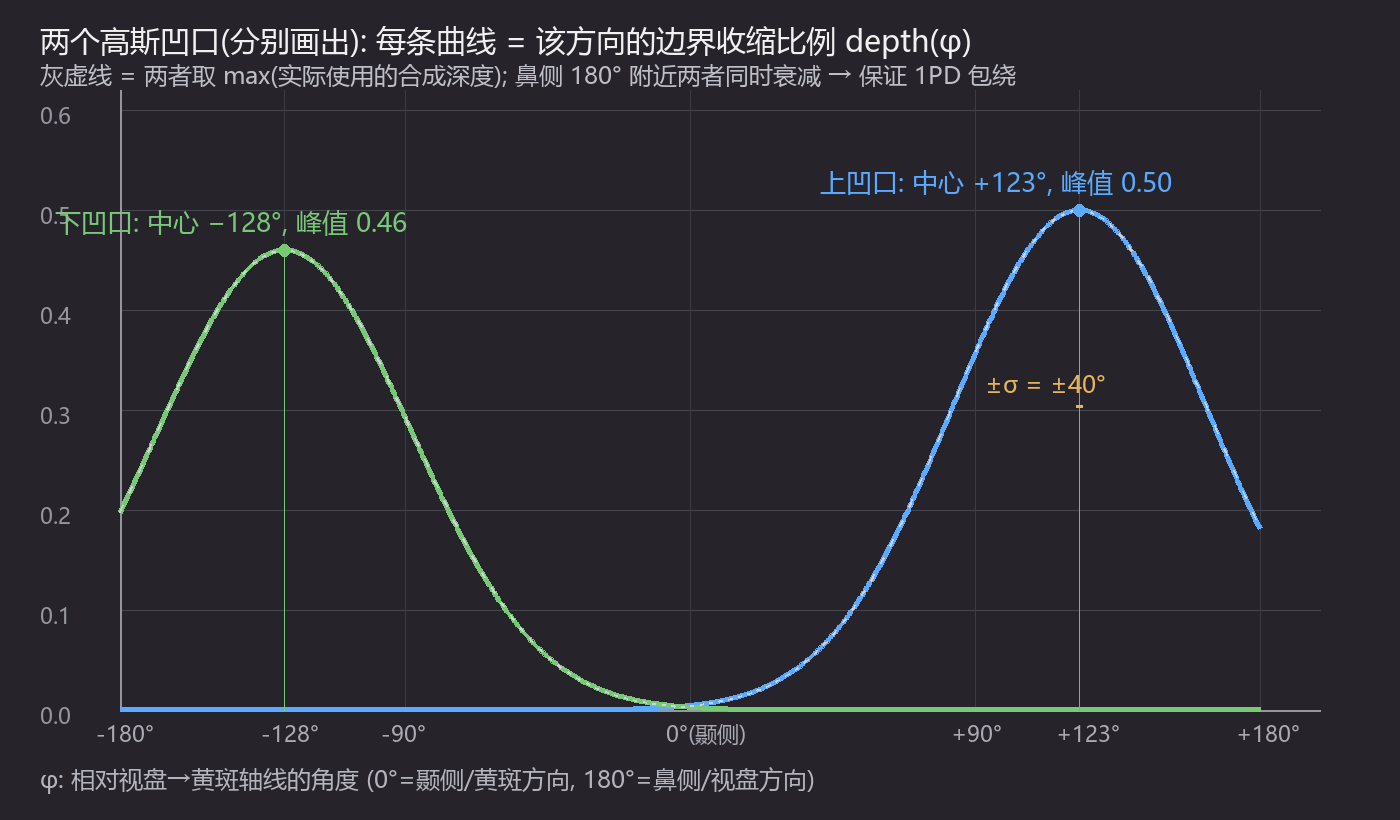
\includegraphics[width=0.98\linewidth]{fig8_notches.png}
\caption{上、下凹口分别画出：蓝线 = 上凹口
$d_{sup}\,e^{-(\varphi-a_{sup})^2/2\sigma^2}$（中心 $+123^\circ$，峰值 0.50），
绿线 = 下凹口 $d_{inf}\,e^{-(\varphi-a_{inf})^2/2\sigma^2}$
（中心 $-128^\circ$，峰值 0.46）。灰虚线 = 两者取 max（实际合成深度）。
在鼻侧（$180^\circ$）附近两条曲线同时衰减，从而保证视盘包绕余量不被侵蚀。}
\end{figure}

\begin{figure}[H]\centering
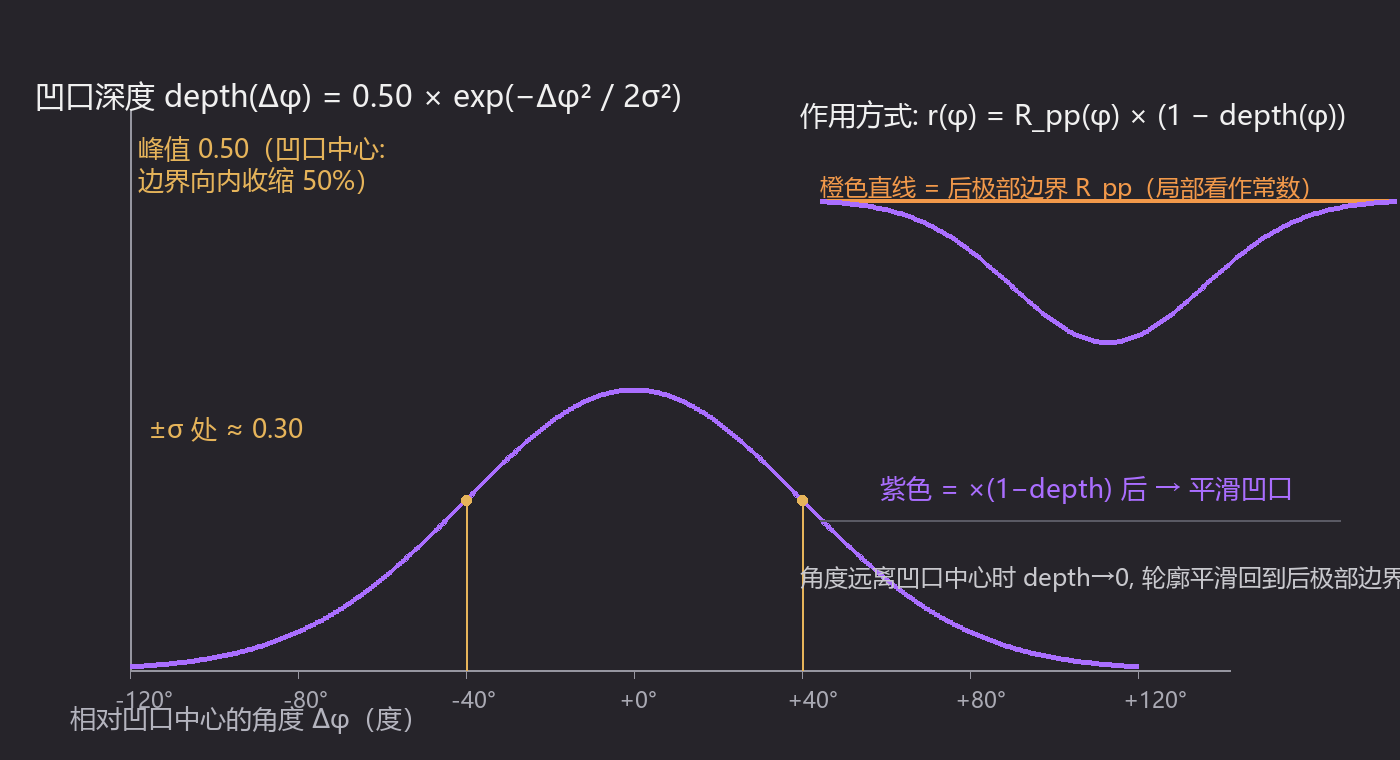
\includegraphics[width=0.95\linewidth]{fig7_gaussian.png}
\caption{高斯凹口原理。左：深度曲线 depth$(\Delta\varphi)$；
右：它如何把后极部边界"压"出平滑凹口。}
\end{figure}

\subsection{鼻侧底噪扣除：保住鼻侧 1\,PD 余量}

两个高斯凹口的尾部会``漏''到鼻方向：在鼻极（$180^\circ$）处，两条尾部合计残留约
20\% 的收缩深度，若不处理会把鼻侧 1\,PD 外扩线向内侵蚀约 $0.2\,a_n$。实现中先按
$180^\circ-a_{sup}$ 与 $180^\circ+a_{inf}$ 计算尾部在鼻极的残留深度
（\texttt{nasal\_depth\_floor}，默认参数下 $\approx 0.198$），再在鼻极方向按
$\sigma_n = 30^\circ$ 的高斯权重将其从 $d(\varphi)$ 中扣除并截断到 $0$。
扣除后鼻极处 $d \to 0$，轮廓贴回后极部卵圆（即鼻侧 1\,PD 外扩线），
鼻侧余量完整保留；两条轮廓仅在鼻极附近分离，其余方向重合。

\begin{figure}[H]\centering
\includegraphics[width=0.98\linewidth]{fig9_nasal_floor.png}
\caption{鼻侧底噪扣除对比（上：眼底鼻侧局部；下：径向剖面）。
青虚线 = 未扣除底噪，鼻侧被高斯尾部向内侵蚀（样例 0003\_3 约 $1.1$ 视盘半径）；
紫粗线 = 软件实际输出，鼻极处贴回 1\,PD 外扩线。}
\end{figure}

\subsection{视盘包绕气泡 $r_{bub}(\varphi)$：保证包住视盘}

以视盘中心为圆心、半径 $= R_d + 1\,\mathrm{PD}$ 的圆。取式~\eqref{eq:main}
的 max 保证无论凹口多深，视盘边缘外永远保留至少 1\,PD 的完整包绕，
且鼻侧前端是圆润的帽而非尖角。

\begin{figure}[H]\centering
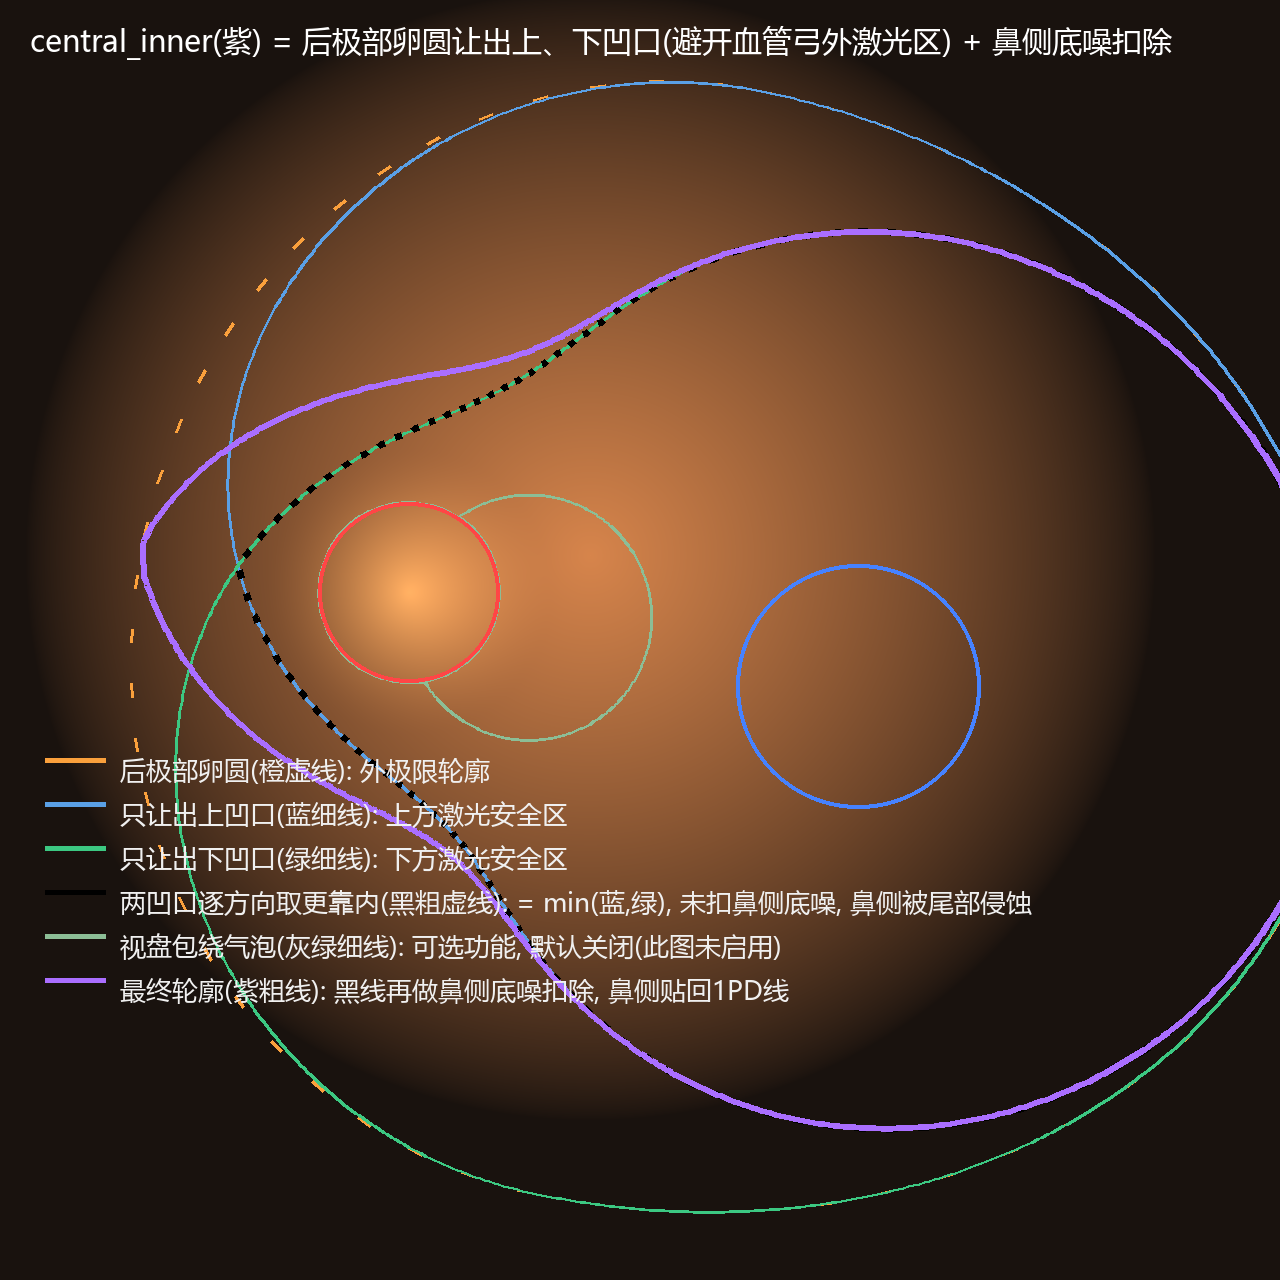
\includegraphics[width=0.9\linewidth]{fig4_construction.png}
\caption{构造分解（在眼底图上）：橙虚线 = 后极部卵圆（外极限轮廓）；
蓝细线 = 只让出上凹口后的轮廓（上方激光安全区）；绿细线 = 只让出下凹口后的轮廓
（下方激光安全区）；黑粗虚线 = 蓝/绿两线\textbf{逐方向取更靠内}的结果
（即逐点 min：上段贴蓝、下段贴绿，鼻侧仍被尾部侵蚀）；
灰绿细线 = 视盘包绕气泡（可选，默认关闭）；
紫粗线 = 最终 central\_inner：在黑线（min）基础上\textbf{再}做鼻侧底噪扣除
（见``鼻侧底噪扣除''一节），鼻侧段贴回 1\,PD 外扩线。}
\end{figure}

\begin{figure}[H]\centering
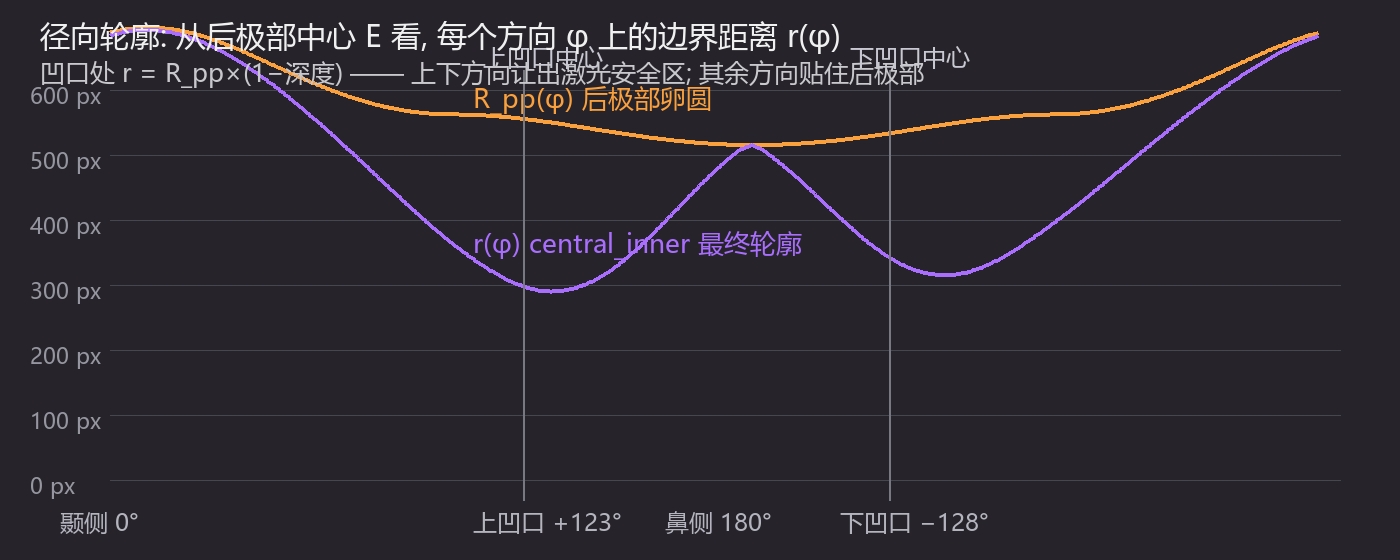
\includegraphics[width=0.95\linewidth]{fig5_profile.png}
\caption{径向剖面 $r(\varphi)$：橙色为后极部卵圆，紫色为最终轮廓。
凹口中心分别位于 $+123^\circ$ 与 $-128^\circ$，鼻侧（$180^\circ$）
与颞侧（$0^\circ$）贴住后极部。}
\end{figure}

\section{参数与标定}

所有默认值由\textbf{组内 14 例手绘标注}自动拟合（Nelder--Mead 最小二乘，
目标为算法轮廓与手绘多边形的双向平均边界距离）：

\begin{center}
\begin{tabular}{llll}
\toprule
参数 & 默认值 & 含义 & 14 例拟合（中位数 $\pm$ std）\\
\midrule
$k_{pp}^{temporal}$ & 2.0 PD & 后极部颞侧外扩 & 按约定固定 \\
$k_{pp}^{nasal}$ & 1.0 PD & 后极部鼻侧外扩 & 按约定固定 \\
$k_{pp}^{vertical}$ & 2.0 PD & 后极部上下外扩 & 按约定固定 \\
$k_{mac}$ & 0.85 & 黄斑圆半径系数 & $0.84 \pm 0.22$ \\
$d_{sup}$ & 0.50 & 上凹口深度比例 & $0.50 \pm 0.06$ \\
$d_{inf}$ & 0.46 & 下凹口深度比例 & $0.46 \pm 0.05$ \\
$\sigma$ & $40^\circ$ & 凹口平滑度（高斯 $\sigma$） & $39.5^\circ \pm 4.8^\circ$ \\
$a_{sup}$ & $123^\circ$ & 上凹口中心角 & $122.7^\circ \pm 9.7^\circ$ \\
$a_{inf}$ & $-128^\circ$ & 下凹口中心角 & $-127.7^\circ \pm 12.9^\circ$ \\
\bottomrule
\end{tabular}
\end{center}

参数间偏差很小，说明该模型稳定复现了手绘约定。与手绘对比的定量结果
（\texttt{scripts/validate\_against\_jsons.py}）：

\begin{itemize}
\item 后极部边界：中位对称距离 \textbf{0.36} 视盘半径；
\item central\_inner：中位对称距离 \textbf{0.39} 视盘半径；
\item 参照：手绘折线自身顶点间距约 1 视盘半径，即算法已达到手绘噪声水平。
\end{itemize}

\begin{figure}[H]\centering
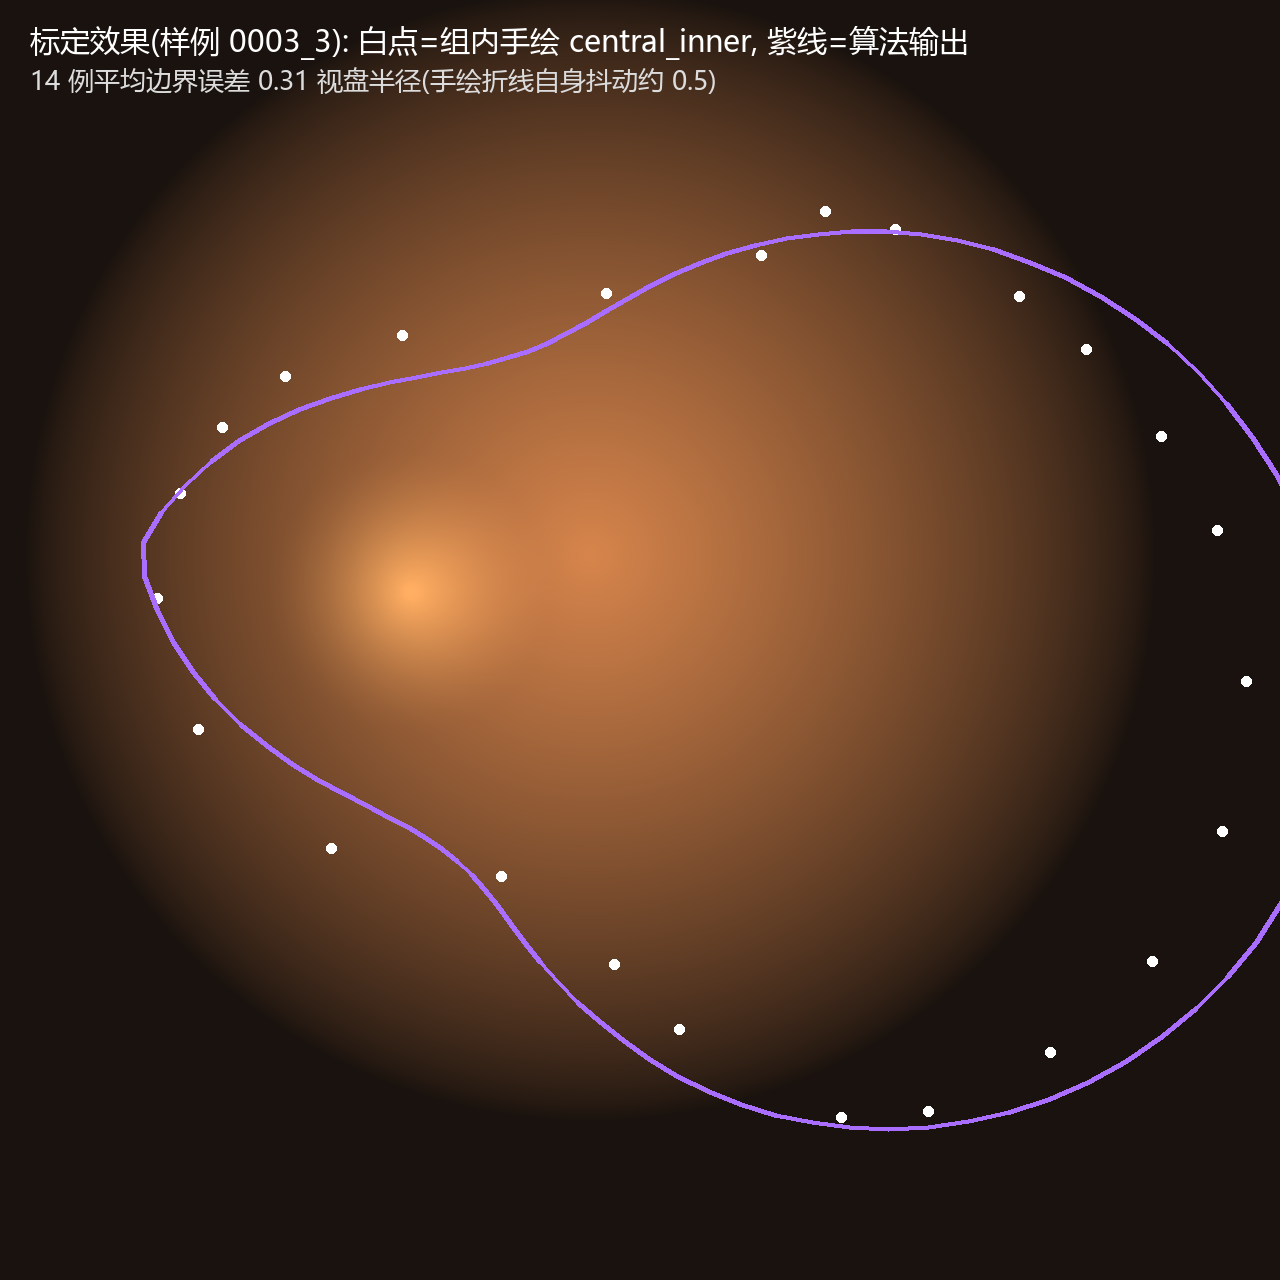
\includegraphics[width=0.8\linewidth]{fig6_calibration.png}
\caption{标定效果（样例 0003\_3）：白点 = 组内手绘 central\_inner，紫线 = 算法输出。}
\end{figure}

\paragraph{为何统一默认值}手绘折线只有 24--35 个顶点，顶点间距约 1 视盘半径，
单例拟合抖动大于参数间差异；统一默认值保证全组标注一致性，个体差异由医生拖点微调。

\section{交互编辑与重算}

\begin{itemize}
\item 视盘 / 黄斑 / 后极部为原生圆形或三点椭圆：拖中心移动、拖边缘/轴端点改变大小与旋转；
\item central\_inner 为 96 点多边形，支持\textbf{平滑变形拖拽}：拖动一点，
周边约 1/5 周长的点按高斯权重平滑跟随，无需逐点调整；
\item 修改视盘 / 黄斑圆后按 \texttt{Ctrl+3} 用新圆重新派生三个结构；
\item \texttt{DR 参数…} 对话框可修改全部派生参数，改后 \texttt{Ctrl+3} 生效；
\item 撤销（Ctrl+Z）与 LabelMe JSON 保存照常可用；AI 生成的结构
\texttt{description} 标记为 \texttt{auto} / \texttt{auto(low-conf)}。
\end{itemize}

\section{代码索引}

\begin{center}
\begin{tabular}{ll}
\toprule
文件 & 内容 \\
\midrule
\texttt{labelmyeye/dr\_geometry.py} & 全部几何：相切椭圆、后极部卵圆、central\_inner 径向模型 \\
\texttt{labelmyeye/auto\_annotate.py} & 点击 $\to$ 分割 $\to$ 圆 $\to$ 五结构的编排 \\
\texttt{labelmyeye/sam\_seg.py} & MobileSAM ONNX 推理与圆拟合 \\
\texttt{scripts/make\_algorithm\_figures.py} & 生成本文档全部插图 \\
\texttt{scripts/calibrate\_fit\_notch.py} & 凹口参数标定（14 例） \\
\texttt{scripts/validate\_against\_jsons.py} & 与手绘标注的定量对比 \\
\texttt{scripts/test\_dr\_geometry.py} & 几何单元测试 \\
\bottomrule
\end{tabular}
\end{center}

\end{document}
